% ============================================================
% Diagrama de Flujo del Sistema Inteligente de Riego
% Vaccinium corymbosum -- Costa de Lima, Peru
% UNMSM -- Facultad de Ingenieria de Sistemas e Informatica
%
% Compilar con: pdflatex diagrama_flujo_sistema.tex
% ============================================================
\documentclass[landscape]{article}
\usepackage[a3paper, margin=1.2cm, top=1.5cm, bottom=1.0cm]{geometry}
\usepackage[utf8]{inputenc}
\usepackage[T1]{fontenc}
\usepackage{amsmath}
\usepackage{helvet}
\renewcommand{\familydefault}{\sfdefault}
\usepackage{tikz}
\usetikzlibrary{
  shapes.geometric,
  shapes.symbols,
  arrows.meta,
  positioning,
  fit,
  backgrounds,
  calc,
  shadows,
  decorations.pathreplacing,
  decorations.markings,
  patterns
}

% ---- Paleta de colores ----------------------------------------
\definecolor{F1col}{HTML}{1565C0}    % Azul  -- Adquisicion
\definecolor{F2col}{HTML}{6A1B9A}    % Morado -- IA
\definecolor{F3col}{HTML}{1B5E20}    % Verde  -- Decision
\definecolor{F4col}{HTML}{BF360C}    % Naranja -- Actuacion

\definecolor{F1bg}{HTML}{DDEEFF}
\definecolor{F2bg}{HTML}{EDE7F6}
\definecolor{F3bg}{HTML}{E8F5E9}
\definecolor{F4bg}{HTML}{FBE9E7}

\definecolor{sensor}{HTML}{0277BD}
\definecolor{esp32}{HTML}{00695C}
\definecolor{firebase}{HTML}{E65100}
\definecolor{mlcolor}{HTML}{6A1B9A}
\definecolor{mamdani}{HTML}{880E4F}
\definecolor{deccolor}{HTML}{2E7D32}
\definecolor{relaycolor}{HTML}{BF360C}
\definecolor{streamcolor}{HTML}{01579B}
\definecolor{watercolor}{HTML}{006064}

% ---- Estilos de nodos -----------------------------------------
\tikzset{
  %-- Hardware / Sensores
  sensor/.style={
    rectangle, rounded corners=6pt,
    draw=sensor, line width=1.2pt,
    fill=sensor!12,
    text width=3.8cm, align=center,
    font=\small\bfseries\color{sensor!70!black},
    inner sep=7pt, minimum height=1.1cm
  },
  esp/.style={
    rectangle, rounded corners=6pt,
    draw=esp32, line width=1.4pt,
    fill=esp32!12,
    text width=3.8cm, align=center,
    font=\small\bfseries\color{esp32!80!black},
    inner sep=7pt, minimum height=1.1cm
  },
  trigger/.style={
    ellipse,
    draw=F1col, line width=1.4pt,
    fill=F1col!10,
    text width=3.4cm, align=center,
    font=\small\bfseries\color{F1col!80!black},
    inner sep=6pt
  },
  %-- Software / API
  process/.style={
    rectangle, rounded corners=6pt,
    draw=mlcolor, line width=1.4pt,
    fill=mlcolor!10,
    text width=4.2cm, align=center,
    font=\small\bfseries\color{mlcolor!80!black},
    inner sep=8pt, minimum height=1.2cm
  },
  mlbox/.style={
    rectangle, rounded corners=6pt,
    draw=mlcolor, line width=1.6pt,
    fill=mlcolor!16,
    text width=4.0cm, align=center,
    font=\small\bfseries\color{mlcolor!80!black},
    inner sep=8pt, minimum height=1.3cm
  },
  mamdanibox/.style={
    rectangle, rounded corners=6pt,
    draw=mamdani, line width=1.6pt,
    fill=mamdani!12,
    text width=4.0cm, align=center,
    font=\small\bfseries\color{mamdani!80!black},
    inner sep=8pt, minimum height=1.3cm
  },
  %-- Decision
  decnode/.style={
    diamond, aspect=2.4,
    draw=deccolor, line width=1.6pt,
    fill=deccolor!12,
    text width=2.6cm, align=center,
    font=\small\bfseries\color{deccolor!80!black},
    inner sep=4pt
  },
  decresult/.style={
    rectangle, rounded corners=5pt,
    draw=deccolor, line width=1.2pt,
    fill=deccolor!10,
    text width=3.4cm, align=center,
    font=\small\bfseries\color{deccolor!70!black},
    inner sep=6pt, minimum height=1cm
  },
  %-- Base de datos
  dbnode/.style={
    cylinder, shape border rotate=90,
    draw=firebase, line width=1.4pt,
    fill=firebase!12,
    text width=2.8cm, align=center,
    font=\small\bfseries\color{firebase!80!black},
    inner sep=6pt, minimum height=1cm,
    aspect=0.3
  },
  %-- Actuacion / Hardware salida
  relay/.style={
    rectangle, rounded corners=6pt,
    draw=relaycolor, line width=1.4pt,
    fill=relaycolor!12,
    text width=3.8cm, align=center,
    font=\small\bfseries\color{relaycolor!80!black},
    inner sep=7pt, minimum height=1.1cm
  },
  valve/.style={
    rectangle, rounded corners=6pt,
    draw=relaycolor!70!black, line width=1.6pt,
    fill=relaycolor!20,
    text width=3.8cm, align=center,
    font=\small\bfseries\color{relaycolor!80!black},
    inner sep=7pt, minimum height=1.1cm
  },
  stream/.style={
    rectangle, rounded corners=6pt,
    draw=streamcolor, line width=1.4pt,
    fill=streamcolor!10,
    text width=3.8cm, align=center,
    font=\small\bfseries\color{streamcolor!80!black},
    inner sep=7pt, minimum height=1.1cm
  },
  water/.style={
    rectangle, rounded corners=6pt,
    draw=watercolor, line width=1.6pt,
    fill=watercolor!12,
    text width=3.8cm, align=center,
    font=\small\bfseries\color{watercolor!80!black},
    inner sep=8pt, minimum height=1.2cm
  },
  %-- Anotaciones
  annot/.style={
    rectangle, rounded corners=3pt,
    draw=gray!50, fill=yellow!15,
    text width=3.2cm, align=center,
    font=\scriptsize\itshape\color{gray!70!black},
    inner sep=5pt
  },
  notelabel/.style={
    font=\scriptsize\color{gray!60!black},
    align=center
  },
  %-- Flechas
  arr/.style={-{Stealth[length=7pt]}, line width=1.4pt, draw=#1},
  arrdash/.style={-{Stealth[length=6pt]}, line width=1pt, draw=#1, dashed},
  labelarr/.style={font=\scriptsize\bfseries, fill=white, inner sep=2pt}
}

\begin{document}
\pagestyle{empty}

\begin{center}

% ---- Titulo principal ----------------------------------------
{\Large\bfseries Sistema Inteligente de Riego --- \textit{Vaccinium corymbosum}}\\[4pt]
{\normalsize Diagrama de Flujo Completo del Sistema (CRISP-DM $\cdot$ Edge AI $\cdot$ IoT)}\\[2pt]
{\small UNMSM -- Facultad de Ingenier\'ia de Sistemas e Inform\'atica $\cdot$ Lima, Per\'u}

\vspace{6pt}

% =============================================================
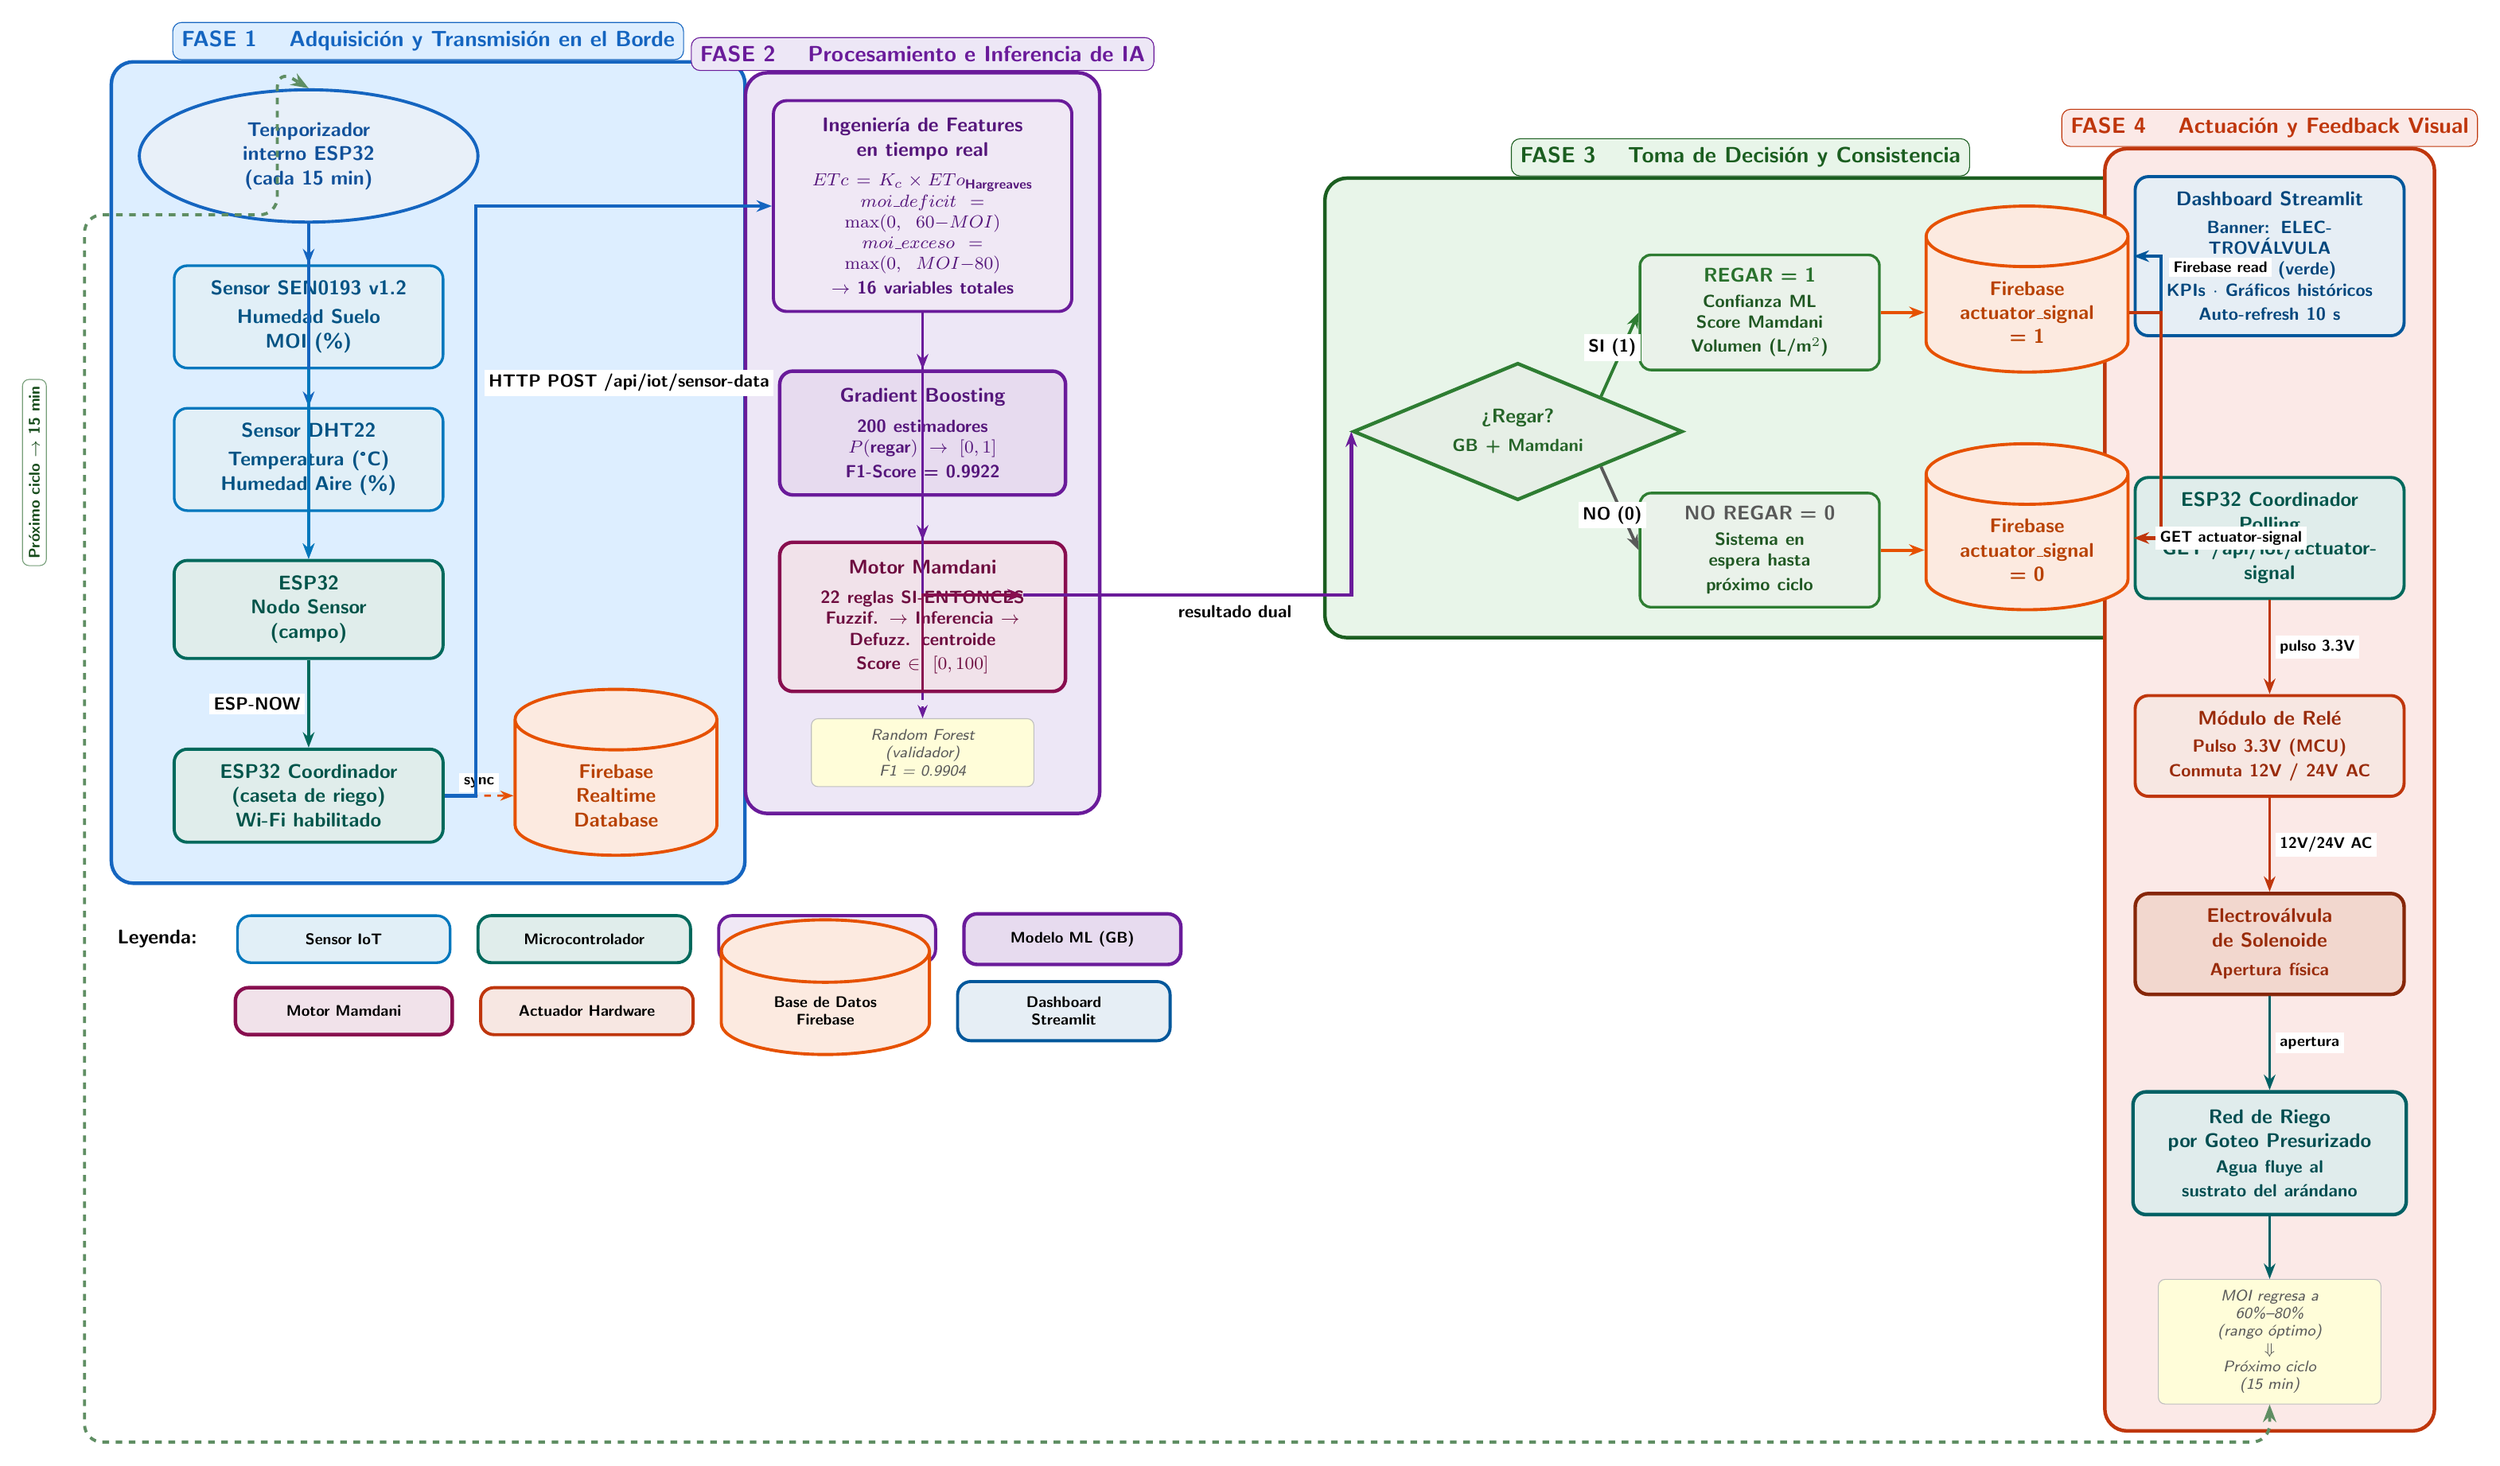
\begin{tikzpicture}[node distance=0.7cm]

% =============================================================
% COLUMNAS X (centros de cada fase)  -- espaciado generoso para A3
%   F1: 3.2    F2: 13.0    F3: 22.5    F4: 34.5
% =============================================================

% ============================================================
%  FASE 1 -- ADQUISICION Y TRANSMISION EN EL BORDE
% ============================================================

\node[trigger] (timer) at (3.2, -1.4)
  {Temporizador\\interno ESP32\\(cada 15 min)};

\node[sensor, below=0.65cm of timer] (sen0193)
  {Sensor SEN0193 v1.2\\[2pt]Humedad Suelo\\MOI (\%)};

\node[sensor, below=0.60cm of sen0193] (dht22)
  {Sensor DHT22\\[2pt]Temperatura ({\textdegree}C)\\Humedad Aire (\%)};

\node[esp, below=0.75cm of dht22] (espnodo)
  {ESP32\\Nodo Sensor\\(campo)};

\node[esp, below=1.4cm of espnodo] (espcoord)
  {ESP32 Coordinador\\(caseta de riego)\\Wi-Fi habilitado};

% Firebase en la columna 1 (lado derecho)
\node[dbnode, right=1.1cm of espcoord] (firebase1)
  {Firebase\\Realtime\\Database};

% ============================================================
%  FASE 2 -- PROCESAMIENTO E INFERENCIA IA
%  X desplazada a 13.0 para separar del cilindro firebase1
% ============================================================

\node[process, align=center] (features) at (13.0, -2.2)
  {Ingenier\'ia de Features\\en tiempo real\\[4pt]
   \footnotesize
   $ETc = K_c \times ETo_{\text{Hargreaves}}$\\
   $moi\_deficit = \max(0,\;60{-}MOI)$\\
   $moi\_exceso = \max(0,\;MOI{-}80)$\\
   $\rightarrow$ 16 variables totales};

\node[mlbox, below=0.9cm of features] (gb)
  {Gradient Boosting\\[4pt]
   \footnotesize
   200 estimadores\\
   $P(\text{regar}) \rightarrow [0,1]$\\
   F1-Score = 0.9922};

\node[mamdanibox, below=0.7cm of gb] (mamdani)
  {Motor Mamdani\\[4pt]
   \footnotesize
   22 reglas SI-ENTONCES\\
   Fuzzif. $\rightarrow$ Inferencia $\rightarrow$\\
   Defuzz. centroide\\
   Score $\in [0,100]$};

% Random Forest: anotacion debajo del gb para no invadir F3
\node[annot, below=0.4cm of mamdani] (rf)
  {Random Forest\\(validador)\\F1 = 0.9904};

% ============================================================
%  FASE 3 -- TOMA DE DECISION
%  X desplazada a 22.5 para separar de la anotacion rf
% ============================================================

\node[decnode] (decision) at (22.5, -5.8)
  {\textbf{?`Regar?}\\[2pt]\footnotesize GB + Mamdani};

\node[decresult, above right=0.4cm and 0.6cm of decision] (regar1)
  {\textcolor{deccolor!90!black}{REGAR = 1}\\[2pt]
   \footnotesize Confianza ML\\Score Mamdani\\Volumen (L/m$^2$)};

\node[decresult, below right=0.4cm and 0.6cm of decision] (noregar)
  {\textcolor{gray!70!black}{NO REGAR = 0}\\[2pt]
   \footnotesize Sistema en\\espera hasta\\pr\'oximo ciclo};

% Firebase: actuator_signal
\node[dbnode, right=0.7cm of regar1] (firebase2)
  {Firebase\\actuator\_signal\\= 1};

\node[dbnode, right=0.7cm of noregar] (firebase3)
  {Firebase\\actuator\_signal\\= 0};

% ============================================================
%  FASE 4 -- ACTUACION Y FEEDBACK VISUAL
%  X desplazada a 34.5 (+8.5 respecto original) para despejar
%  firebase2/firebase3 de la caja F4.
%  Apilado interno con below=1.5cm para evitar solapamientos.
% ============================================================

% -- Rama visual (Streamlit) --
\node[stream] (streamlit) at (34.5, -3.0)
  {Dashboard Streamlit\\[3pt]
   \footnotesize
   Banner: ELECTROV\'ALVULA\\ACTIVA (verde)\\
   KPIs $\cdot$ Gr\'aficos hist\'oricos\\
   Auto-refresh 10 s};

% -- Rama hardware: apilado con below=1.5cm --
\node[esp] (esppoll) at (34.5, -7.5)
  {ESP32 Coordinador\\Polling\\GET /api/iot/actuator-signal};

\node[relay, below=1.5cm of esppoll] (relay)
  {M\'odulo de Rel\'e\\[3pt]
   \footnotesize
   Pulso 3.3V (MCU)\\
   Conmuta 12V / 24V AC};

\node[valve, below=1.5cm of relay] (valve)
  {Electrov\'alvula\\de Solenoide\\[2pt]\footnotesize Apertura f\'isica};

\node[water, below=1.5cm of valve] (water)
  {Red de Riego\\por Goteo Presurizado\\[2pt]
   \footnotesize Agua fluye al\\sustrato del ar\'andano};

% -- Loop de cierre --
\node[annot, below=1.0cm of water] (loop)
  {MOI regresa a\\60\%--80\%\\(rango \'optimo)\\$\Downarrow$\\Pr\'oximo ciclo\\(15 min)};

% =============================================================
%  FONDOS DE FASE (dibujados con begin{scope})
% =============================================================
\begin{scope}[on background layer]

  % FASE 1
  \node[
    fit=(timer)(espcoord)(firebase1),
    fill=F1bg, draw=F1col, line width=1.6pt,
    rounded corners=10pt, inner sep=12pt,
    label={[anchor=south, font=\normalsize\bfseries\color{F1col},
            fill=F1bg, draw=F1col, rounded corners=4pt,
            inner sep=4pt]north:
            {FASE 1 \quad Adquisici\'on y Transmisi\'on en el Borde}}
  ] (boxF1) {};

  % FASE 2
  \node[
    fit=(features)(gb)(mamdani)(rf),
    fill=F2bg, draw=F2col, line width=1.6pt,
    rounded corners=10pt, inner sep=12pt,
    label={[anchor=south, font=\normalsize\bfseries\color{F2col},
            fill=F2bg, draw=F2col, rounded corners=4pt,
            inner sep=4pt]north:
            {FASE 2 \quad Procesamiento e Inferencia de IA}}
  ] (boxF2) {};

  % FASE 3
  \node[
    fit=(decision)(regar1)(noregar)(firebase2)(firebase3),
    fill=F3bg, draw=F3col, line width=1.6pt,
    rounded corners=10pt, inner sep=12pt,
    label={[anchor=south, font=\normalsize\bfseries\color{F3col},
            fill=F3bg, draw=F3col, rounded corners=4pt,
            inner sep=4pt]north:
            {FASE 3 \quad Toma de Decisi\'on y Consistencia}}
  ] (boxF3) {};

  % FASE 4
  \node[
    fit=(streamlit)(esppoll)(relay)(valve)(water)(loop),
    fill=F4bg, draw=F4col, line width=1.6pt,
    rounded corners=10pt, inner sep=12pt,
    label={[anchor=south, font=\normalsize\bfseries\color{F4col},
            fill=F4bg, draw=F4col, rounded corners=4pt,
            inner sep=4pt]north:
            {FASE 4 \quad Actuaci\'on y Feedback Visual}}
  ] (boxF4) {};

\end{scope}

% =============================================================
%  FLECHAS INTERNAS -- FASE 1
% =============================================================

\draw[arr=F1col] (timer) -- (sen0193);
\draw[arr=F1col] (timer) -- (dht22);

% Sen0193 y DHT22 convergen al nodo sensor
\draw[arr=sensor] (sen0193) -- (espnodo);
\draw[arr=sensor] (dht22)   -- (espnodo);

% ESP-NOW
\draw[arr=esp32] (espnodo) --
  node[labelarr, left=1pt] {\footnotesize ESP-NOW}
  (espcoord);

% Firebase sync (desde coordinador)
\draw[arrdash=firebase] (espcoord) --
  node[labelarr, above=1pt] {\scriptsize sync}
  (firebase1);

% =============================================================
%  FLECHAS ENTRE FASES 1 -> 2
% =============================================================

\draw[arr=F1col, line width=1.6pt]
  (espcoord.east) -- ++(0.5,0) |-
  node[labelarr, pos=0.35, right=3pt]
    {\footnotesize HTTP POST /api/iot/sensor-data}
  (features.west);

% =============================================================
%  FLECHAS INTERNAS -- FASE 2
% =============================================================

\draw[arr=F2col] (features) -- (gb);
\draw[arr=F2col] (features) -- (mamdani);

% RF como validador (debajo de mamdani)
\draw[arrdash=mlcolor] (mamdani.south) -- (rf.north);

% GB y Mamdani convergen al pipeline de decision
\coordinate (merge) at ($(gb.south)!0.5!(mamdani.south)$);
\coordinate (mergeOut) at ($(merge) + (1.6, 0)$);

\draw[arr=mlcolor]   (gb.south)      |- (mergeOut);
\draw[arr=mamdani]   (mamdani.south) |- (mergeOut);

% =============================================================
%  FLECHAS ENTRE FASES 2 -> 3
% =============================================================

\draw[arr=F2col, line width=1.6pt]
  (mergeOut) -- ++(0.6,0) -|
  node[labelarr, pos=0.3, below=2pt]
    {\footnotesize resultado dual}
  (decision.west);

% =============================================================
%  FLECHAS INTERNAS -- FASE 3
% =============================================================

\draw[arr=deccolor]
  (decision.north east) -- (regar1.west)
  node[labelarr, pos=0.3, above=4pt] {\footnotesize SI (1)};

\draw[arr=gray!70!black]
  (decision.south east) -- (noregar.west)
  node[labelarr, pos=0.3, below=4pt] {\footnotesize NO (0)};

\draw[arr=firebase] (regar1.east)  -- (firebase2.west);
\draw[arr=firebase] (noregar.east) -- (firebase3.west);

% =============================================================
%  FLECHAS ENTRE FASES 3 -> 4
% =============================================================

% Firebase2 (signal=1) -> Streamlit (via Firebase read)
\draw[arr=streamcolor, line width=1.4pt]
  (firebase2.east) -- ++(0.5,0) |-
  node[labelarr, pos=0.4, right=3pt]
    {\scriptsize Firebase read}
  (streamlit.west);

% Firebase2 (signal=1) -> ESP32 Polling
\draw[arr=F4col, line width=1.6pt]
  (firebase2.east) -- ++(0.5,0) |-
  node[labelarr, pos=0.75, right=3pt]
    {\scriptsize GET actuator-signal}
  (esppoll.west);

% =============================================================
%  FLECHAS INTERNAS -- FASE 4 (hardware)
% =============================================================

\draw[arr=relaycolor] (esppoll) --
  node[labelarr, right=2pt] {\scriptsize pulso 3.3V}
  (relay);

\draw[arr=relaycolor] (relay) --
  node[labelarr, right=2pt] {\scriptsize 12V/24V AC}
  (valve);

\draw[arr=watercolor] (valve) --
  node[labelarr, right=2pt] {\scriptsize apertura}
  (water);

\draw[arr=watercolor] (water) -- (loop);

% =============================================================
%  FLECHA DE RETROALIMENTACION (loop de cierre)
% =============================================================

\draw[{Stealth[length=8pt]}-{Stealth[length=8pt]},
      line width=1.4pt, draw=F3col!70, dashed, rounded corners=8pt]
  (loop.south) -- ++(0,-0.6) -| ($(boxF1.south west) + (-0.4,-0.3)$)
  -- ++(0, 11) -| ($(timer.north) + (-0.5, 0.3)$) -- (timer.north);
\node[font=\scriptsize\bfseries\color{F3col!80!black},
      fill=white, inner sep=3pt, draw=F3col!60, rounded corners=3pt]
  at ($(boxF1.west) + (-1.2, 0)$) [rotate=90]
  {Pr\'oximo ciclo $\rightarrow$ 15 min};

% =============================================================
%  LEYENDA  --  2 filas x 4 columnas
% =============================================================

\node[anchor=north west, font=\small\bfseries]
  at ($(boxF1.south west) + (0,-0.6)$) (legTitle) {Leyenda:};

% --- Fila 1 ---
\node[sensor, text width=2.9cm, minimum height=0.75cm,
      font=\scriptsize\bfseries,
      right=0.5cm of legTitle, anchor=west] (l1) {Sensor IoT};

\node[esp, text width=2.9cm, minimum height=0.75cm,
      font=\scriptsize\bfseries,
      right=0.4cm of l1, anchor=west] (l2) {Microcontrolador};

\node[process, text width=2.9cm, minimum height=0.75cm,
      font=\scriptsize\bfseries,
      right=0.4cm of l2, anchor=west] (l3) {Proceso de Software};

\node[mlbox, text width=2.9cm, minimum height=0.75cm,
      font=\scriptsize\bfseries,
      right=0.4cm of l3, anchor=west] (l4) {Modelo ML (GB)};

% --- Fila 2 (justo debajo de fila 1) ---
\node[mamdanibox, text width=2.9cm, minimum height=0.75cm,
      font=\scriptsize\bfseries,
      below=0.35cm of l1, anchor=north] (l5) {Motor Mamdani};

\node[relay, text width=2.9cm, minimum height=0.75cm,
      font=\scriptsize\bfseries,
      right=0.4cm of l5, anchor=west] (l6) {Actuador Hardware};

\node[dbnode, text width=2.9cm, minimum height=0.75cm,
      font=\scriptsize\bfseries,
      right=0.4cm of l6, anchor=west] (l7) {Base de Datos\\Firebase};

\node[stream, text width=2.9cm, minimum height=0.75cm,
      font=\scriptsize\bfseries,
      right=0.4cm of l7, anchor=west] (l8) {Dashboard\\Streamlit};

\end{tikzpicture}

\end{center}
\end{document}
